% Chapter Template

\chapter{Literature Review} % Main chapter title

\label{LiteratureReview} % Change X to a consecutive number; for referencing this chapter elsewhere, use \ref{ChapterX}

%----------------------------------------------------------------------------------------
%	SECTION 1
%----------------------------------------------------------------------------------------

While much of recent deep learning research has focused on developing novel architectures and specialized modules, there has been comparatively little investigation into the role of dense and flexible connectivity within neural networks. Existing work often explores new types of connections or processing blocks, such as attention mechanisms~\cite{vaswani2017attention}, MLP Mixers~\cite{tolstikhin2021mlp}, and Convolutional blocks~\cite{krizhevsky2012imagenet}, but rarely addresses the fundamental question of how increasing connection density itself could impact learning capacity and model performance.

This chapter begins with an overview of the field of Neural Architecture Search (NAS), discussing its objectives, prevalent techniques, and its influence on neural network optimization. The review then covers the classical MLP framework, pruning methods—including the influential Lottery Ticket Hypothesis—and other architectural innovations relevant to the development and motivation of Sarosh’s Perceptron Networks (SPNs). Together, these topics provide the theoretical and practical context for the proposed research and its contributions.



\section{Neural Architecture Search (NAS)}

Neural Architecture Search (NAS) is an automated method for optimizing neural network architectures. The primary objective of NAS is to find an optimal architecture that provides the best trade-off between model performance (accuracy) and resource usage (computational efficiency, parameter count, and memory usage) \cite{elsken2019neural}. NAS has significantly contributed to the advancement of deep learning by automating architecture design, traditionally a manually intensive process.

\begin{figure}[h!]
    \centering
    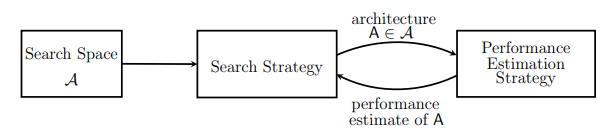
\includegraphics[width=1.0\textwidth]{Literature Review/abstract_nas_search_methods.png}
    \caption{An abstract illustration of NAS~\cite{elsken2019neural} Search Methods.}
    \label{fig:abstractNASMethods}
\end{figure}

%-----------------------------------
%	SUBSECTION 1
%-----------------------------------
\subsection{Current Techniques in NAS}

NAS techniques are broadly categorized into reinforcement learning (RL)-based methods, evolutionary algorithms (EA), and gradient-based optimization methods.

\textbf{Reinforcement Learning-based NAS} techniques use an RL agent that generates neural architectures and updates its strategy based on rewards from evaluating the architectures \cite{zoph2016neural}. Notable examples include the work by Zoph and Le, where an RNN controller designs neural architectures \cite{zoph2016neural}.

\textbf{Evolutionary Algorithm-based NAS} methods use population-based optimization inspired by biological evolution, including mutation, crossover, and selection to evolve architectures \cite{real2019regularized}. Real et al. demonstrated that evolutionary methods could effectively evolve architectures that outperform manually designed ones \cite{real2019regularized}.

\textbf{Gradient-based NAS} methods, such as Differentiable Architecture Search (DARTS), formulate NAS as a continuous optimization problem, allowing for efficient gradient-based optimization \cite{liu2018darts}. DARTS has become popular due to its efficiency in discovering competitive architectures with lower computational cost.

\begin{table}[ht]
\centering
\caption{Comparison of NAS Techniques}
\begin{tabular}{|c|c|c|}
\hline
\textbf{Technique} & \textbf{Advantages} & \textbf{Disadvantages} \\
\hline
RL-based & High flexibility & Computationally expensive \\
\hline
EA-based & Effective global search & Requires extensive evaluations \\
\hline
Gradient-based & Efficient and scalable & Sensitive to initialization \\
\hline
\end{tabular}
\label{tab:nas_techniques}
\end{table}

%----------------------------------------------------------------------------------------
%	SECTION 2
%----------------------------------------------------------------------------------------

\section{Multi-Layer Perceptrons (MLPs)}
Multi-Layer Perceptrons (MLPs) are classical feedforward artificial neural networks composed of multiple layers of nodes (neurons). Each neuron employs a non-linear activation function enabling the network to learn complex patterns through supervised learning techniques, such as backpropagation \cite{rumelhart1986learning}. MLPs have traditionally served as baseline models due to their simplicity and general applicability across diverse tasks, including classification and regression problems.

\begin{figure}[h!]
    \centering
    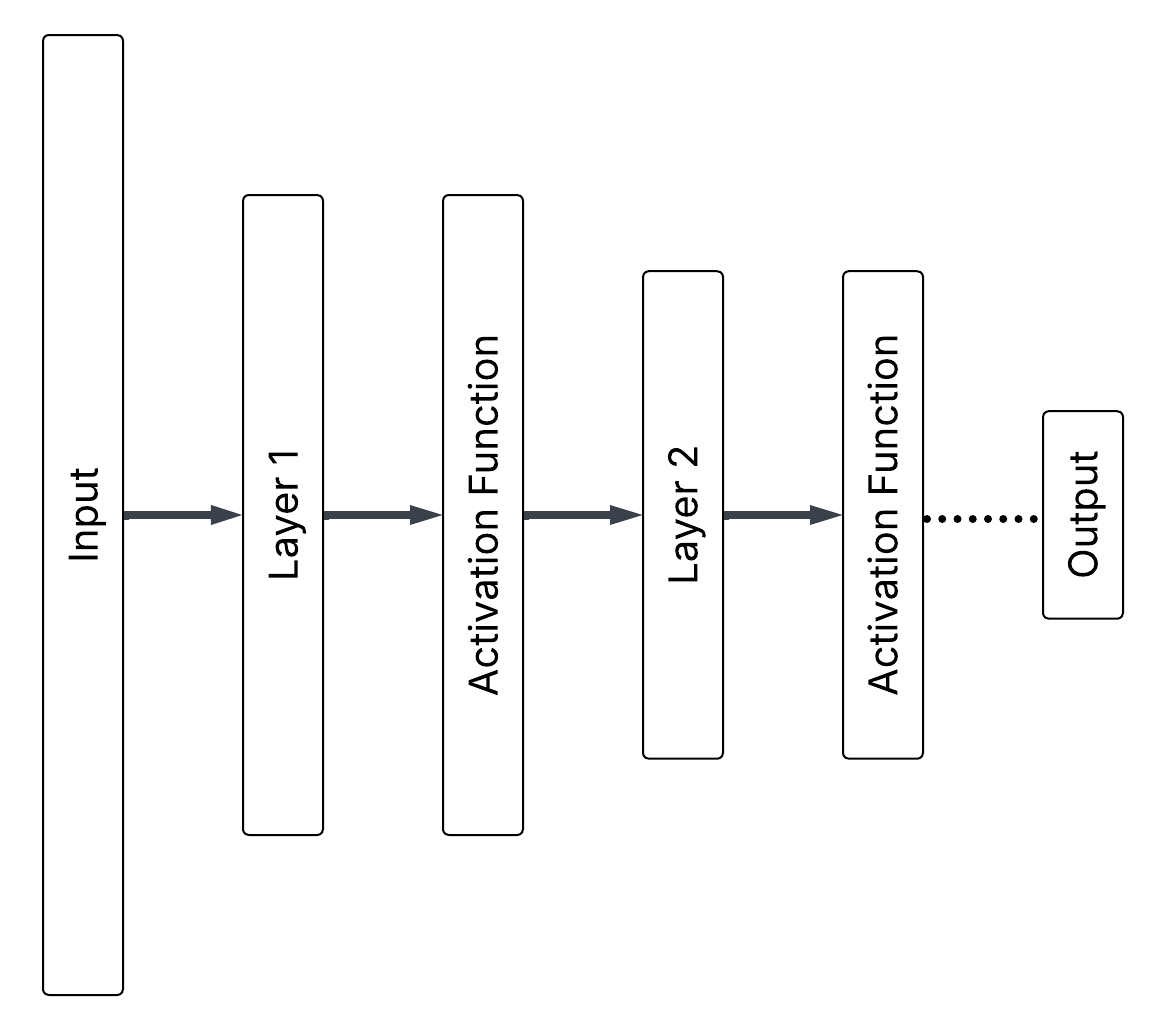
\includegraphics[width=0.6\textwidth]{Literature Review/example_MLP_architecture.png}
    \caption{An example MLP Architecture.}
    \label{fig:exampleMLP}
\end{figure}

However, MLPs typically suffer from issues such as overfitting and computational inefficiency when scaling to deeper and wider networks. This motivates research into improving the architectural efficiency and effectiveness of MLPs through enhanced connectivity, optimized neuron allocation, and specialized training procedures.

\section{Residual Networks (ResNets)}

Residual Networks (ResNets), introduced by He et al.~\cite{he2016deep}, represent a significant breakthrough in deep learning by enabling the effective training of very deep neural networks. ResNets address the vanishing gradient problem, a phenomenon where gradients become exceedingly small as they are backpropagated through many layers, hindering learning in deep architectures, by introducing residual connections. A residual connection, or skip connection, allows the input of a layer (or a set of layers) to be added directly to the output, thereby forming a shortcut path for the gradient during backpropagation. 

Formally, for a given input $\mathbf{x}$ and a residual function $F(\mathbf{x})$, the output of a residual block is $\mathbf{y} = F(\mathbf{x}) + \mathbf{x}$. Importantly, these connections do not introduce new trainable weights for the shortcut path; instead, they simply sum the input and the output of the residual block, providing a form of informed augmentation rather than increasing connectivity in the traditional sense. For residual addition to be valid, the dimensions of the input and output must match; when they do not, projection shortcuts with $1 \times 1$ convolutions are used to adjust dimensions. 

\begin{figure}[h!]
    \centering
    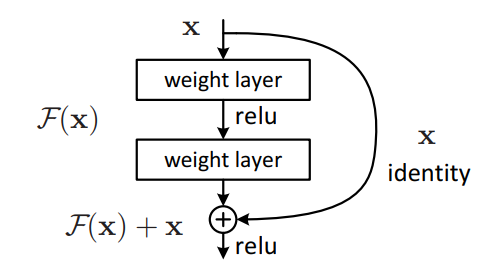
\includegraphics[width=0.6\textwidth]{Literature Review/example_residual_block.png}
    \caption{Example of a residual block in ResNets~\cite{he2016deep}.}
    \label{fig:exampleResNet}
\end{figure}


Furthermore, residual connections are typically local, linking only layers that are one or two steps apart, while more distant neurons remain disconnected. Thus, although ResNets represent a major advance in making deep learning practical and effective, they do not fundamentally expand the overall connectivity space of the network, but rather improve information and gradient flow through carefully structured local augmentations.


\section{Pruning in Neural Networks}
Pruning is a method to reduce network complexity by eliminating redundant connections or neurons, effectively improving computational efficiency without significantly compromising performance \cite{han2015learning}. It seeks to achieve sparsity within the network, reducing the model size, memory footprint, and inference latency, thus facilitating deployment in resource-constrained environments.

Pruning methods can be classified into magnitude-based, structure-based, and learning-based pruning:

\textbf{Magnitude-based pruning} involves removing weights based on their absolute magnitude, assuming low-magnitude weights contribute less to the network's predictive capability \cite{han2015learning}.

\textbf{Structured pruning} removes entire channels or layers, maintaining regular structure beneficial for hardware acceleration \cite{he2017channel}.

\textbf{Learning-based pruning}, such as iterative magnitude pruning, incrementally prunes the network while retraining it to recover accuracy \cite{han2015learning}.

\section{Lottery Ticket Hypothesis}
The Lottery Ticket Hypothesis, proposed by Frankle and Carbin, posits that dense, randomly-initialized neural networks contain smaller subnetworks (winning tickets often as small as less than 10\% the size of the original network) which, when trained in isolation, can match or exceed the test accuracy of the original network \cite{frankle2018lottery}.

This hypothesis suggests that initialization plays a crucial role in neural network training. Frankle and Carbin’s pruning approach involves:
\begin{enumerate}
\item Training the original network fully.
\item Pruning a fraction of the lowest magnitude weights.
\item Resetting the remaining weights to their initial values.
\item Repeating this iterative process multiple times.
\end{enumerate}

The Lottery Ticket Hypothesis has provided a theoretical and empirical foundation for understanding network pruning and initialization strategies. It emphasizes the importance of structured pruning approaches, challenging the traditional random pruning practices.

\section{Summary}
This literature review highlights the advancements in neural architecture optimization through NAS, the foundational structure and limitations of MLPs and ResNets, and the efficacy of pruning methods, particularly through the lens of the Lottery Ticket Hypothesis. These areas collectively inform strategies for improving neural network performance and efficiency, forming the theoretical underpinning of this thesis.